\subsection{Microcontroller}
To implement the controller digitally an microcontroller (MCU) was required to carry out the computations. In addition to interfacing with external peripheral circuitry, the MCU has four main responsibilities that include:
\begin{itemize}
    \item Measurement of the input and output voltages of the \'Cuk Converter.
    \item Calculation of control action.
    \item Generating switching signal for the converter.
    \item Communication with host machine.
\end{itemize}
The calculations required for the control algorithm are computationally expensive and must be executed online (that is computed in real time rather than pre-computed offline). This type of computation is well suited to a digital signal processors (DSP).
\\ \\
The MCU was carefully chosen such that as many of the critical components were included as peripherals rather than requiring external components. This saved board space and allowed for a less complicated design, it also saved time as it removed the need to interface with the components using serial communication protocols. The main peripherals required were a fast ADC at a high resolution in addition to DAC that supported PWM at the high frequencies to allow for smaller components.
\\ \\
Microchip's dsPIC33EP ``GS'' series of specialised digital signal controllers are designed for high-speed digital control loops and contained the additional peripherals for interfacing with external circuitry. Specifically the \texttt{dsPIC33EP64GS504} was chosen, as it also contained a number of peripherals tailed for switched mode power supply control.
\begin{figure}
    \centering
    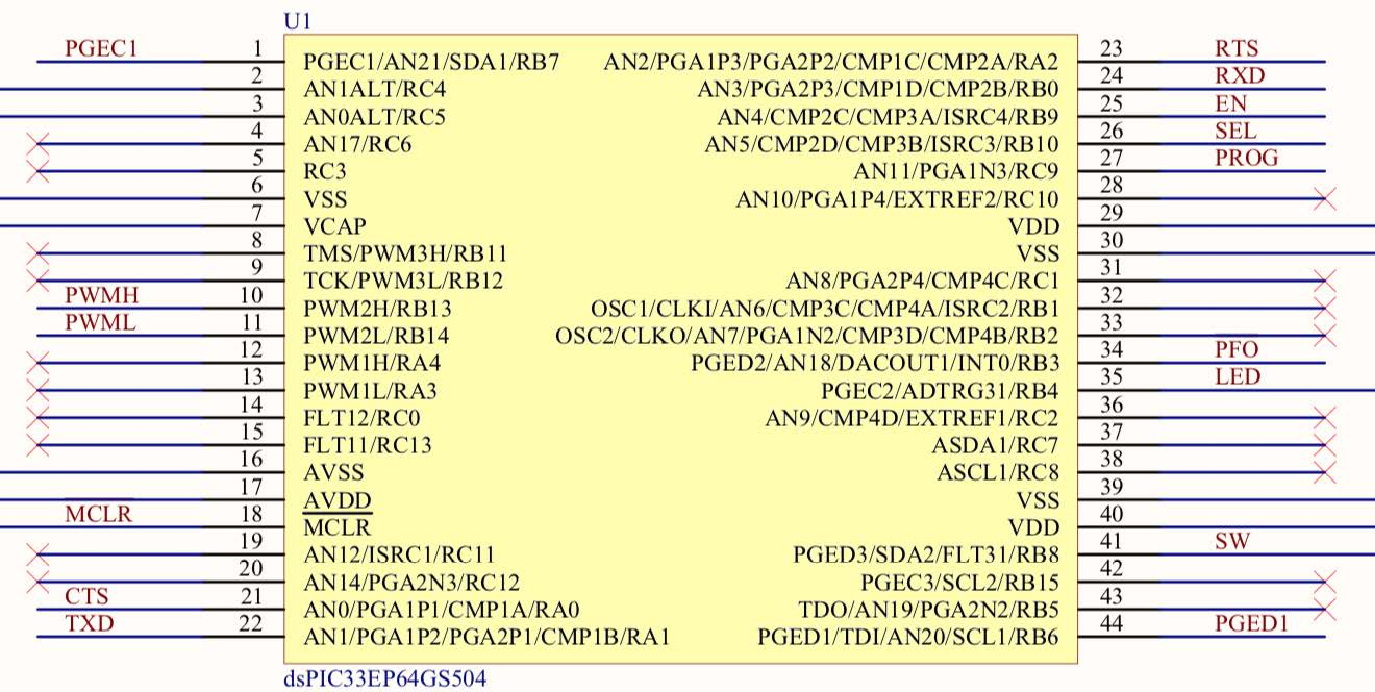
\includegraphics[height = 8cm]{figures/hardware/mcu_schematic.pdf}
    \caption{MCU schematic excerpt.}
    \label{fig:mcu_schematic}
\end{figure}
Operating at a clock rate of \SI{120}{MHz}, the MCU is capable of \SI{60}{MIPS}. This is generated using the internal fast RC oscillator (FRC) that provides a nominal \SI{7.37}{MHz} clock. As this is a RC oscillator, timer accuracy would be limited and affected by a number of external factors (such as temperature). However as the sampling rate was chosen to be \SI{10}{kHz} (section \ref{sec:system_params}) the presence of jitter proved not to affect the performance of the converter. An external clock could be used for addition precision, it was decided to avoid including this in the initial design as it would complicated the PCB layout as well and increasing the time required to write firmware for the device.
%%%%%%%%%%%%%%%%%%%%%%%%%%%%%%%%%%%%%%%%%%%%%%%%%%%%%%%%%%%%%%%%%%%%%%%%%%%%%%%%
\subsubsection{Analog-to-digital converter (ADC)}
The \texttt{dsPIC33EP64GS504} contained an high-speed ADC module was several desirable features:
\begin{itemize}
    \item Four dedicated SAR cores each configurable for up to 12-bits of resolution. This feature was central in the choice of the micro controller as it allowed for the simultaneous measurements of all four of the \'Cuk converter states if observer implementation proved to be difficult or the execution speed was too slow.
    \item Up to 3.25 Msps conversion rate per channel at 12-bit resolution, when using a \SI{70}{MHz} instruction clock.
    \item Flexible and independent ADC trigger sources that allow for minimal CPU interaction, allowing the ADC to run independently while the costly control algorithm is computed.
\end{itemize}

\paragraph{Successive approximation register (SAR) ADC}
Conversion of the continuous analog signal into a discrete digital representation occurs via a binary search. Through the use of a digital-to-analog converter the ADC generates a reference voltage and compares it to the analog voltage that was sampled. For each of the 16-bits of digital data (starting with the most significant bit) the SAR compares if the voltage is higher or lower than the voltage generated by the data, eventually converging on the final quantisation level and generating the 16-bit digital word \cite{sar_adc}.
\\ \\
SAR ADCs are inherently slow due to the nature of the algorithm that they implement, as the algorithm must narrow in on the voltage over a number of stages that scales with the number of bits used in the representation. The rate at which conversions occur is directly coupled to the instruction clock. For maximum conversion rate the instruction clock should be configured to be as high as possible. For ideal performance the ADC must convert the signal instantaneously at the start of the sampling interval. To approximate this the conversion time should be approximately an order of magnitude smaller than the sampling period. Since \SI{10}{kHz} was chosen for the sampling rate, and a \SI{60}{MHz} instruction clock was used, the ADC conversion rate is 620ns. This is much smaller than the sampling period of 20us and hence approximately occurred instantaneously.
%%%%%%%%%%%%%%%%%%%%%%%%%%%%%%%%%%%%%%%%%%%%%%%%%%%%%%%%%%%%%%%%%%%%%%%%%%%%%%%%
\subsubsection{Pulse width modulation (PWM)}
A single fast PWM module was sued to send switching signal to the DC-DC converter. PWM signal was configured to run at \SI{10}{kHz} and duty cycle is controlled by writing to a register, PDC1. 
%%%%%%%%%%%%%%%%%%%%%%%%%%%%%%%%%%%%%%%%%%%%%%%%%%%%%%%%%%%%%%%%%%%%%%%%%%%%%%%%
\subsubsection{Timer}
A single 16-bit timer module was used to implement the sampling rate of converter. ADC triggering was against this timer to ensure sampling occurred at the start of each interval. Controller computations were also executed within this sampling period.

\subsubsection{Programmer}
An in-circuit serial programmer (ICSP) was used for debugging and flashing of microcontroller firmware. The Microchip \textit{PICkit\textsuperscript{TM} 3 In-Circuit Debugger} was untilised and require six connections via a standard header on the PCB, see appendix \ref{apn:pcb}.